% Diese Zeile bitte -nicht- aendern.
\documentclass[course=erap]{aspdoc}

%%%%%%%%%%%%%%%%%%%%%%%%%%%%%%%%%
%% TODO: Ersetzen Sie in den folgenden Zeilen die entsprechenden -Texte-
%% mit den richtigen Werten.
\newcommand{\theGroup}{146} % Beispiel: 42
\newcommand{\theNumber}{A217} % Beispiel: A123
\author{Giancarlo Calvache \and Vlad-Alexandru Marin \and Emre Öztas}
\date{Wintersemester 2022/23} % Beispiel: Wintersemester 2019/20
%%%%%%%%%%%%%%%%%%%%%%%%%%%%%%%%%

% Diese Zeile bitte -nicht- aendern.
\title{Gruppe \theGroup{} -- Abgabe zu Aufgabe \theNumber}

\begin{document}
\maketitle

\section{Einleitung}

Diese Ausarbeitung befasst sich mit der computergestützten Darstellung des \emph{Burning-Ship} Fraktals, einer modifizierten Version des \emph{Mandelbrot} Fraktals.
Fraktale\cite{FractalGeometry} sind geometrische Objekte und Muster, die auf allen Größenskalen \emph{selbstähnlich} sind und deren Komplexität nie zu Ende geht. Der Begriff wurde 1975 vom Vater der fraktalen Geometrie \emph{Benoit Mandelbrot} ins Leben gerufen und leitet sich vom Lateinischem Wort Fractus, im Deutschen "gebrochen", ab. Die Geometrie der Frakale wurde als Antwort auf die Frage eingeführt, wie man die allgegenwärtige Komplexität der in der Natur vorkommenden Gegenstände, wie die Äste von Bäumen, Blütenstrukturen oder Küstenlinien, in einer geometrischen Formulierung schematisieren kann.
\newline
Oftmals, entstehen Darstellungen von Fraktalen durch einfache Rekursions- oder Iterationsvorschriften, welche ein komplexes Muster erzeugen. Die Art und Weise, wie ein Fraktal vom Computer erzeugt wird, ist dabei eng gekoppelt mit seiner mathematischen Definition. Daher, sind Fraktale lediglich eine verbildlichte Darstellung einer mathematischen Rekursionsformel. Im Fall des \emph{Burning-Ship} Fraktals verwenden wir einen \emph{Escape-Time-Algorithmus}, um zu berechnen, ob ein Punkt sich in der \emph{Burning-Ship}-Menge befindet oder nicht.
\newline
 Eine Implementierung auf Basis von 32-bit single-precision floating points kann nur eine sehr begrenzte Genauigkeit in der Darstellung erzielen. Um eine höhere Genauigkeit zu realisieren, muss die Genauigkeit und damit die Speichergröße der verwendeten floating points gleichermaßen vergrößert werden, was zu einem geringeren Durchsatz in der parallelen Verarbeitung führt.
Aufgrund der beschränkten Registergrößen von Rechnern, ist eine unendlich genaue Berechung von Fraktalen daher impraktikabel, zumindest wenn die Berechung nicht auf Kosten von Performanz und Speichernutzung des Rechners geht. Eine Möglichkeit die Berechung der Iterationsvorschrift zu erleichtern, ist es die Berechung aufzuteilen und jede parallele Verarbeitungseinheit mit der SIMD-Erweiterung zu optimieren. Diese Praxis taucht in moderner Software für die Generierung von Fraktalen auf, würde allerdings den Umfang des Projektes sprengen, da die Arithmetik der erweiterten Floating Points aus den genannten Gründen, angepasst werden müsste.
\newline
Vor diesem Hintergrund ist die Zielsetzung für das Projekt, eine Implementierung für die Iterationsvorschrift des \emph{Burning-Ship} Fraktals zu schreiben, welche anhand Parallelität mittels SSE-CPU-Erweiterungen optimiert ist, und ein Rahmenprogramm zu entwickeln, durch welches das Fraktal in einer festgelegten Auflösung als verlustlose Bilddatei generiert werden kann. Hierzu verwenden wir das kompressionsfreie Format BMP\cite{BMPMedium}\cite{BMPINFOwingdi} mit einer Farbtiefe von 8-bit. Darüberhinaus, wird das Rahmenprogramm durch den
Zusatz erweitert, das Fraktal bis zu 10000-Fach vergrößert erzeugen zu können, um die meist verborgenen Muster innerhalb von Fraktalen ansatzweise sichtbar zu machen.
\newline
Die Entscheidungen und Erwägungen, welche wir für die Implementierung getroffen haben, werden in den nächsten Abschnitten näher erläutert.
\section{Lösungsansatz}

Zur Menge des \emph{Burning-Ship}-Fractals gehören alle Punkte $c = \Re(c) + i * \Im(c) = (\Re(c), \Im(c))$ der Komplexen Ebene im Raum von $[-2, 2]^2 \in \mathbf{R}^2$, die nicht divergieren, wenn die folgende Iterationsvorschrift mit $z_{0} = 0$; $k$-Fach angewendet wird:
\begin{equation}z_{n+1} = (\mid\Re(z_{n})\mid + \mid\Im(z_{n})\mid)^2 + c\end{equation} Wir bezeichnen später $c$ als die Position des Pixel auf einem Bild der Dimension $m \times n$, welches wir erzeugen.
\subsection{Das Rahmenprogramm}
Der Benutzer soll in der Lage sein, einen exakten Punkt auf der \emph{Burning-Ship}-Menge zu fixieren und eine Vergrößerung an der Stelle vorzunehmen. Dies wird durch die beiden Programm-Optionen \emph{-s<Real>,<Imag>} und \emph{-r<Vergrößerungsfaktor>} umgesetzt, wobei alle Argumente dieser Optionen Gleitkommazahlen sind, die eine Präzision von 64-Bit in der Mantisse haben, wodurch etwa 15 Nachkommastellen in Dezimaldarstellung für die Berechnung verwendet werden können. Alle möglichen Eingaben für -s sind auf den oben genannten Raum beschränkt und die Eingaben für -r sind durch das Intervall $[4.0, 1e-15]$ begrenzt. Darüberhinaus soll der Benutzer ebenfalls, die Dimension des Ausgabebildes bestimmen können, was durch die Option \emph{-d<Breite,Höhe>} erfolgt. Da verwertbare Ergebnisse entstehen sollen, wird eine Dimension des Ausgabebildes auf das Intervall $[100, 8000]$ in Pixeln beschränkt, da die Angabe zu kleiner Dimensionen dazu führt, dass das Ergebnis der Iteration nicht wahrnehmbar ist und zu große Dimensionen dazu, dass Bilder mit einer Speichergroße von mehreren Gigabytes erzeugt werden. Zu weiteren Programmargumenten gehören -h bzw. --help, wodurch ein Hilfstext zur Benutzung des Programmes angezeigt wird, -o zum setzten des Namen der Ausgabedatei, -B<Anzahl der Wiederholungen> durch Benchmarks, mit der Angegebenen Anzahl wiederholt werden. Die Option -V<Index> gibt an, welche Implementierung verwendet wird, um das Fraktal zu erzeugen. Es sind die folgenden Implementierungen vordefiniert, welche dem Index nach, beginnend mit Null, sortiert sind:
\begin{enumerate}
    \item burning\_ship \textemdash \; Ohne Optimierungen
    \item burning\_ship\_V1 \textemdash \; SIMD
    \item burning\_ship\_V2 \textemdash \; AVX
\end{enumerate}
Die Option -n<Natürliche Zahl> gibt an, für wie viele Iterationen $k$ die Folge $(z_{n})_{k}$ berechnet wird.


\subsection{Umsetzung der Iterationsvorschrift}

Um zu berechnen ob ein Punkt $c$ auf der Komplexen Ebene gegen unendlich konvergiert oder nicht, oder anders gesagt ob der Punkt die Eigenschaft der Burning-Ship-Menge nicht erfüllt, müssen wir eine Eigenschaft der Komplexen Zahlen finden, welche uns erlaubt diese Invariante effizient zu überprüfen. Ein Beweis \cite{BoundaryTwoProof} zeigt, dass es ausreicht, für Punkte $c_{x,y}$ in einem Bereich der Komplexen Zahlen zu zeigen, dass $c_{x,y}$ genau dann sich nicht in der \emph{Burning-Ship} Menge befindet, wenn ab einer Iteration $k$ gilt, dass $\lVert z_{k} \rVert > 2$. Für ein $c$ mit $\mid\Re(c)\mid > 2$ oder $\mid\Im(c)\mid > 2$ ist dies automatisch der Fall, weshalb wir nur eine Umgebung $c \in [-2, 2]^2$ betrachen müssen. Dazu wandeln wir die Iterationsvorschrift um, in dem wir die Gleichung in (1) auflösen und sie nach dem Real- und Imaginärteil aufschreiben:
\begin{equation}
\Re(z_{n+1}) = \Re(z_{n})^2 - \Im(z_{n})^2 + \Re(c)
\end{equation}
\begin{equation}
\Im(z_{n+1}) = 2\mid\Re(z_{n})\Im(z_{n})\mid + \Im(c)
\end{equation}
Diese beiden Gleichungen werden benötigt, um die Wurzelberechung innerhalb der Vektornorm zu umgehen und stattdessen zu Berechnen ob $\lVert z_{k} \rVert ^ 2 > 4$. Wir bezeichnen jedes Pixel auf dem Ausgabebild als $p_{x,y} \in [0,Breite] \times [0, Hoehe]$. Da die Iterationsfunktion des \emph{Burning-Ship} Fraktals die Farbstufe des Pixels anhand dem oben genannten Raum berechnet d.h. $\Phi_{burning\_ship}(p_{x,y}, n) : ([-2, 2]^2) \times n \rightarrow [0, 1]$, sodass die Koordinate, welche vergrößert werden soll, sich bei Eingabe genau im Mittelpunkt des Bildes befindet, müssen wir zwei Projektionen $\pi_{x}(p_{x,y}) : [0, Breite] \rightarrow [-2,2] \cdot R$ und $\pi_{y}(p_{x,y}) : [0, Hoehe] \rightarrow [-2,2] \cdot R$ definieren, welche die Dimensionen des Bildes in eine geeignete Form umwandeln bevor sie der Iterationsfunktion übergeben werden. $R \in [1, 10^{-6}]$ ist hierbei der Vergrößerungsfaktor des Bildes. Dadurch erhalten wir das folgende Programm, welches das \emph{Burning-Ship} Fraktal mit Angabe der Dimension des Bildes, dem Vergrößerungsfaktor und der Anzahl an Interationen pro Pixel berechnet:

\subsection{Färbung und Schreiben in einem BMP-Datei}
Wir haben eine Farbentabelle erstellt, die im Header der BMP-Datei gelagert wird. Diese Tabelle entsteht aus 16 Farben. Nachdem wir die Anzahl von Iterationen für jede Pixel berechnet haben, skalieren wir diese Nummern im Bereich [0,15]. Die erhaltene Index dient dafür, dass wir für jede Pixel eine Farbe aus der Tabelle zuordnen. Zunächst wird eine BMP-Datei erstellt, die aus dem vordefinierten Header und die Farbenindexe aller Pixeln entsteht.

\begin{figure}[htp]
    \centering
    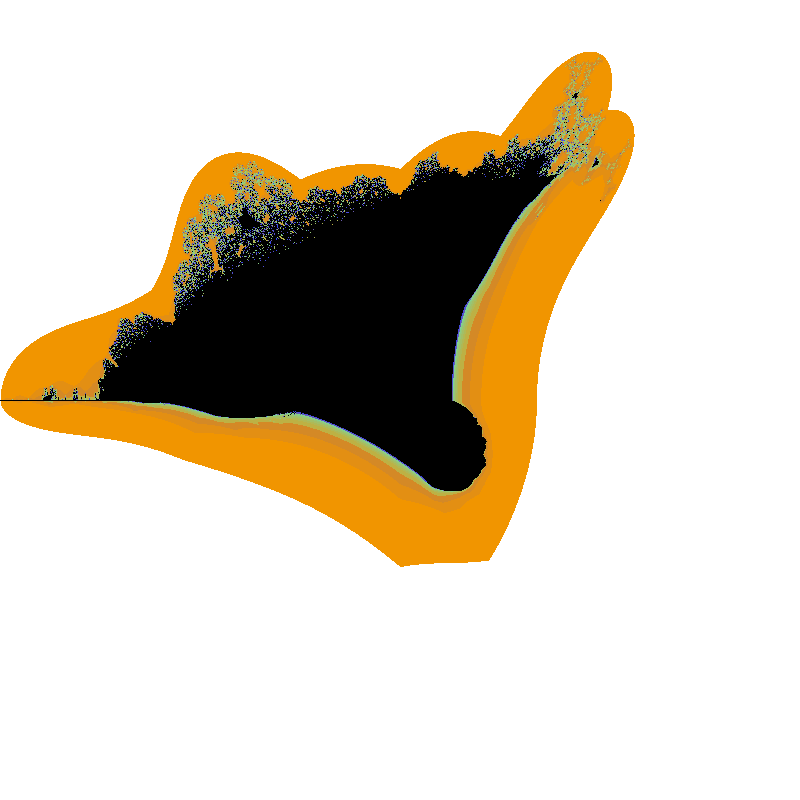
\includegraphics[width=10cm]{Ausarbeitung/bs.png}
    \caption{Größte burning ship mit Parametern -d 800,800 -n 40 -r 4}
    \label{fig:big_ship}
\end{figure}

\section{Genauigkeit}
Wir haben eine Testfunktion implementiert, die die Ausgabe der gegebenen Parameter und Implementierung berechnet. Gleichzeitig wird die SISD-Implementierung mit der gleichen Parameter geruft. Die Ergebnisse werden pixelweise verglichen und das Verhältnis von unterschiedlichen Pixel zu alle Pixel wird ausgegeben. Des Weiteren haben wir die Implementierungen mit verschiedenen Eingaben testet. \ref{tab:table_label}
\begin{table}[h]
\centering
\begin{tabular}{|c|c|c|c|c|c|}
\hline
d & r & s & n & SIMD & AVX \\ [0.5ex] 
\hline\hline
800,800 & 1.0 & 0,0 & 40 & 14.116094\% & 14.116094\% \\
800,800 & 1.0 & 0,0 & 30 &  0.270625\% &  0.270625\% \\ 
800,800 & 1.0 & 0,0 & 50 &  12.767344\% &  12.767344\% \\ 
1000,1000 & 1.0 & 0.0 & 40 & 13.974400\% & 13.974400\% \\
800,800 & 4.0 & 0,0 & 40 & 16.977344\% & 16.977969\% \\
800,800 & 0.1 & 0,0 & 40 & 0\% & 0\% \\
800,800 & 0.009 & -1.77001035,-0.05000005 & 40 & 48.806250\% & 48.881719\% \\ [1ex]
\hline
\end{tabular}
\caption{Fehlerquotioent der Implementierungen}
\label{tab:table_label}
\end{table}

Die Tabelle zeigt den Fehlerquotienten der Implementierungen von SIMD und AVX. Es scheint, dass der Fehlerquotient von verschiedenen Faktoren abhängt, wie z.B. den Werten für d, r, s und n. In einigen Fällen haben beide Implementierungen einen ähnlichen Fehlerquotienten, wie bei 800,800 für d und 40 für n (14.116094\% für SIMD und 14.116094\% für AVX). In anderen Fällen ist der Fehlerquotient Null, wie bei 800,800 für d und 0.1 für r. Allgemein scheint AVX einen geringfügig niedrigeren Fehlerquotienten zu haben als SIMD.

\section{Performanzanalyse}
Wir haben mit verschiedenen Eingaben Laufzeitmessungen durchgeführt. Alle Messungen, die in diesem Unterabschnitt erläutert werden, sind auf einem System mit einem Intel(R) Core(TM) i7-7700K CPU @ 4.20GHz (8 CPUs), ~4.2GHz Prozessor, 16384MB Arbeitsspeicher, Windows 10 Home 64-bit, 256KB L1, 1MB L2 und 8MB L3.

Wir haben in allen Optimierungslevel getestet. Die folgende Abbildungen wurden mit -O3 kompiliert. Abbildung \ref{fig:progressive_n} zeigt, die durchschnittliche Laufzeite von drei verschiedenen Implementierungen, in Abhängigkeit von dem maximalen Anzahl von Iterationen. Abbildung \ref{fig:small_ship} stellt die durchschnittliche Performanze der drei Implementierungen beim \nameref{fig:small_ship}, abhängig von den Dimensionen dar. Die Eingaben sind so gewählt, damit die Performanze bei verschiedenen Bildgrößen und maximale Iterationsschritte deutlich darzustellen
\begin{figure}[htp]
    \centering
    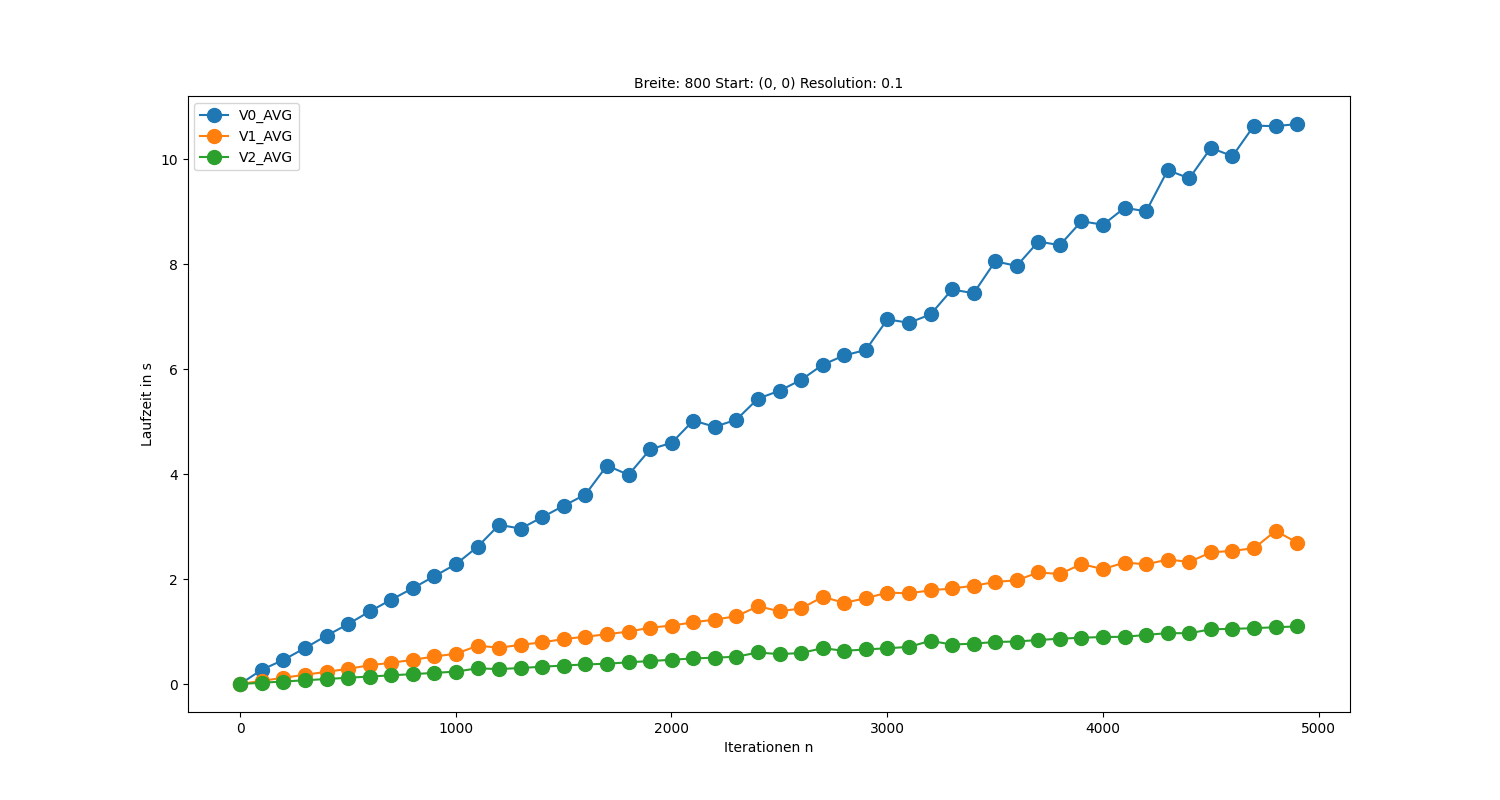
\includegraphics[width=14cm]{Ausarbeitung/progressive_n.png}
    \caption{Progessive n mit B = 5}
    \label{fig:progressive_n}
\end{figure}

\begin{figure}[htp]
    \centering
    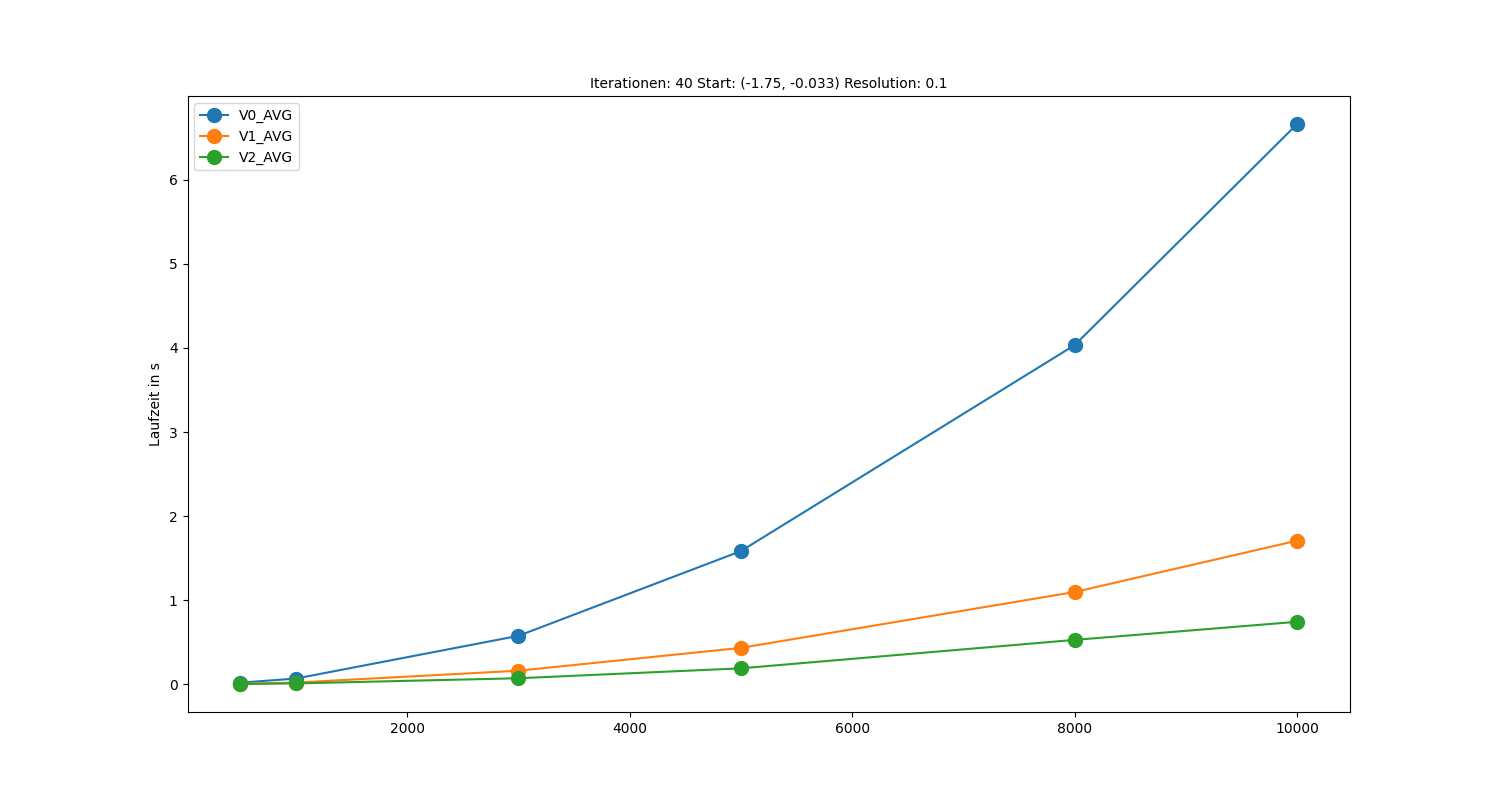
\includegraphics[width=14cm]{Ausarbeitung/Small ship_dot_line.png}
    \caption{\nameref{fig:small_ship} mit B = 5}
    \label{fig:small_ship_graph}
\end{figure}

\begin{figure}[htp]
    \centering
    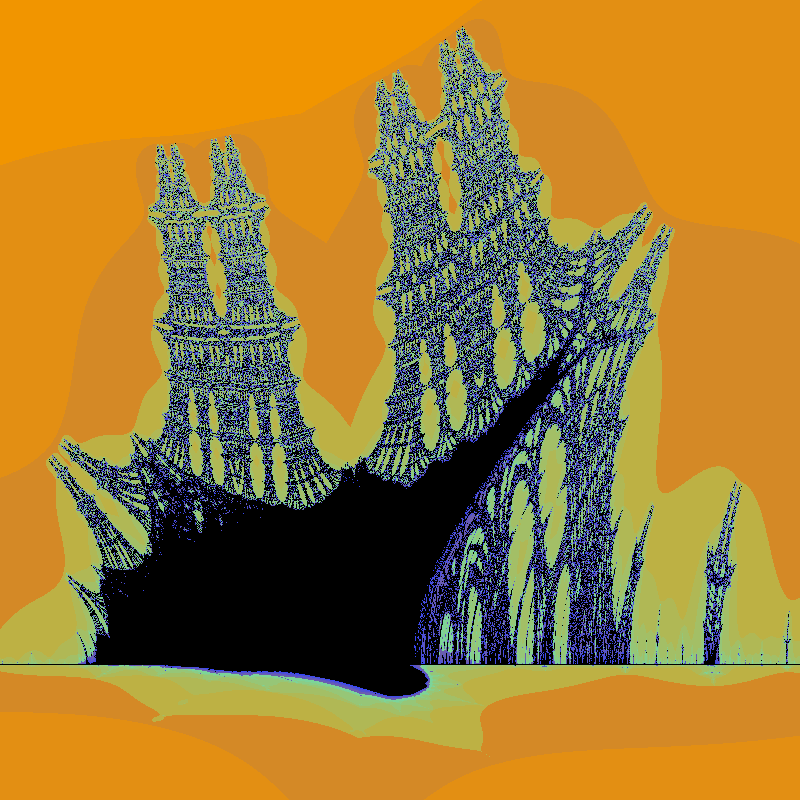
\includegraphics[width=5cm]{Ausarbeitung/small_ship.png}
    \caption{Small Ship}
    \label{fig:small_ship}
\end{figure}

Wenn man den beiden Graphen untersucht, kann man sagen, dass die erste Implementierung langsam ist und eine längere Zeit benötigt, um eine bestimmte Aufgabe auszuführen. Die zweite Implementierung ist schneller als die erste, aber nicht so schnell wie die dritte. Die dritte Implementierung ist die schnellste von allen dreien und benötigt die kürzeste Zeit, um eine Aufgabe auszuführen. Dieses Ergebnis ist erwartet, da V0 1 Pixel, V1 4 Pixel und V2 8 Pixel pro Iterationsschritt überabeitet.

Es ist wichtig zu beachten, dass die Geschwindigkeit einer Implementierung von verschiedenen Faktoren abhängt, wie z.B. der Effizienz des Algorithmus, dem verwendeten Prozessor und dem verwendeten Arbeitsspeicher. Trotzdem kann die schnelle Implementierung ein klarer Vorteil sein, insbesondere wenn es um große Datenmengen oder komplexe Aufgaben geht.

\section{Zusammenfassung und Ausblick}
In diesem Projekt wurde eine Funktion, die den Burning Ship Fraktal erstellt, implementiert. Die Funktion erhält als Parameter den Startpunkt des Ausschnitts, die Breite, die Höhe, die gewünschte Auflösung und die maximale Anzahl der Iterationen. Außerdem wird ein Zeiger auf einen Speicherbereich übergeben, der groß genug ist, um die berechneten Bitmap-Daten des Ergebnisses aufzunehmen. Die Funktion ist so konzipiert, dass sie eine innvolle Farbpalette verwendet, um das Ergebnis darzustellen. In diesem Projekt wurden insgesamt drei Implementierungen erstellt: eine normale Implementierung, eine SIMD-Implementierung und eine AVX-Implementierung. Die haben verschiedene Laufzeitverhältnisse und Genaugkeiten haben.

Eine mögliche Erweiterung des Projektes könnte die Verwendung von GPU-Beschleunigung sein, um die Berechnungsgeschwindigkeit und Effizienz zu verbessern. Es ist auch wichtig, alternative Lösungen zu untersuchen, um Nachteile, wie Korrektheit von V1 und V2 der aktuellen Implementierungen zu erkennen und gegebenenfalls zu verbessern. Zum Beispiel könnte eine alternative Lösung eine höhere Auflösung bei gleichbleibender Geschwindigkeit und Effizienz ermöglichen. Darüber hinaus kann die Vergleichbarkeit der drei Implementierungen weiter untersucht werden, um die beste Option für bestimmte Anwendungsfälle zu bestimmen.

% TODO: Fuegen Sie Ihre Quellen der Datei Ausarbeitung.bib hinzu
% Referenzieren Sie diese dann mit \cite{}.
% Beispiel: CR2 ist ein Register der x86-Architektur~\cite{intel2017man}.
\bibliographystyle{plain}
\bibliography{Ausarbeitung}{}

\end{document}
